% Latex template: mahmoud.s.fahmy@students.kasralainy.edu.eg
% For more details: https://www.sharelatex.com/learn/Beamer

\documentclass{beamer}					  % Document class

\usepackage[portuguese]{babel}			  % Set language
\usepackage[utf8x]{inputenc}			  % Set encoding

\mode<presentation> {					  % Set options
  \usetheme{default}					    % Set theme
  \usecolortheme{default} 				% Set colors
  \usefonttheme{default}  				% Set font theme
  \setbeamertemplate{caption}[numbered]	% Set caption to be numbered
}

\setbeamertemplate{navigation symbols}{}
\setbeamertemplate{footline}[frame number]
\setbeamercovered{transparent}

% Uncomment this to have the outline at the beginning of each section highlighted.
%\AtBeginSection[]
%{
%  \begin{frame}{Outline}
%    \tableofcontents[currentsection]
%  \end{frame}
%}

\usepackage{graphicx}					% For including figures
\usepackage{booktabs}					% For table rules
\usepackage{hyperref}					% For cross-referencing
\usepackage{caption}                    % Allows more control over captions in figs and tables

\title{Revisão de Atividades da FAC}	% Presentation title
%\author{Author One}					% Presentation author
\institute{LNLS.DAC.FAC}				% Author affiliation
\date{2023-10-27 -- 2023-11-17}			% Today's date	


\begin{document}



\begin{frame}
  \titlepage
  \href{https://github.com/lnls-fac/doc-review-dac-fac}{\beamergotobutton{Link para o repo github desta apresentação: https://github.com/lnls-fac/doc-review-dac-fac}}
  \href{https://www.overleaf.com/read/sbdjxtzfchrm}{\beamergotobutton{Link para o projeto overleaf destas notas}}
\end{frame}

\begin{frame}{Outline}
  \tableofcontents
\end{frame}


\section{Atividades - Campo DELTA52 e Calibração modelo RADIA}

\begin{frame}{Calibração do Modelo DELTA52: Motivação}
    \begin{itemize}
		\item A ideia é ter um modelo RADIA 3D do ID que explique as medidas de mapas de campo feitas com sensor Hall, que no caso do DELTA, só podem ser feitas no plano $y = 0$. Com este modelo calibrado podemos fazer RK para resolver a traj. 3D e obter os mapas de kicks transversais $x'(x_0, y_0)$ e $y'(x_0, y_0)$ para estudar o efeito do ID na ótica e abertura dinâmica.
        \item Usando as medidas de mapas de campo com sensor Hall, calibramos o modelo RADIA do ID
        \item Trabalhando para melhorar a calibração do modelo...
	\end{itemize}
\end{frame}

\begin{frame}{Campo DELTA52 e Calibração do modelo}
\begin{itemize}
        \item Campo integrado: modelo calibrado x medidas (antes)
	\end{itemize}
\begin{figure}[H]
		\centering
        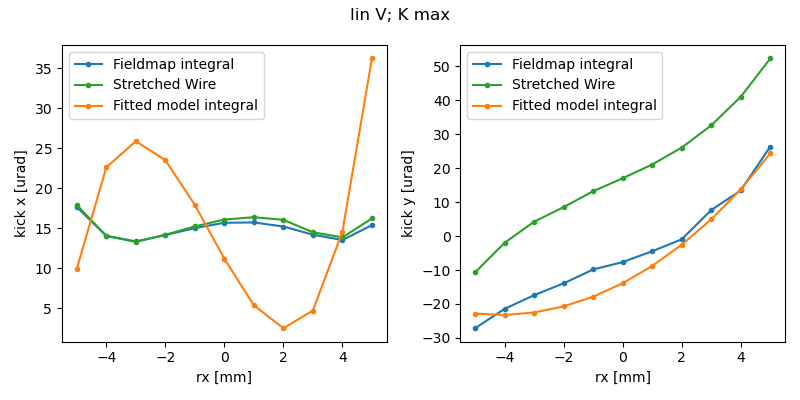
\includegraphics[width=.9\textwidth]{2023-10-27/figures/field_integrals_fitting.png}
        \label{fig:integral_fitting}
    \end{figure}
\end{frame}

\begin{frame}{Calibração do modelo}
    \begin{itemize}
            \item Melhorias no cálculo do jacobiano (alinhamento de grids).
    \end{itemize}
    \begin{figure}[H]
    		\centering
            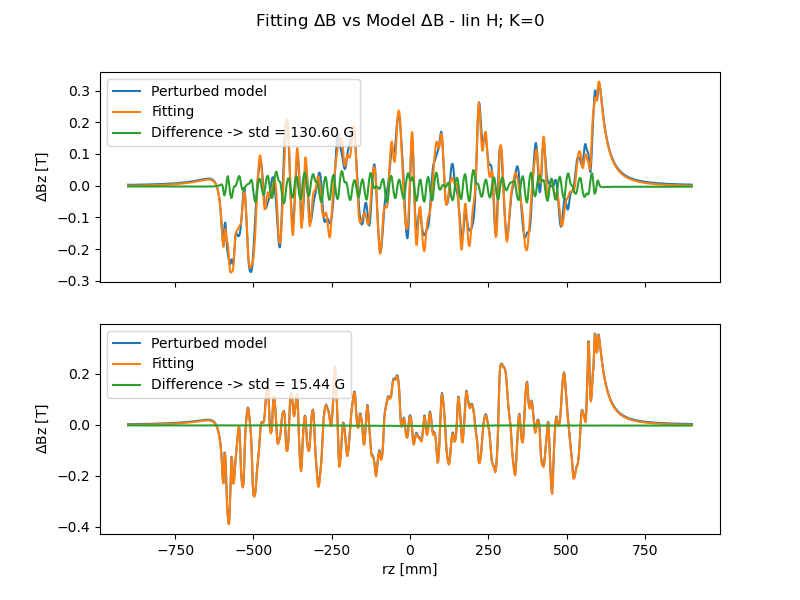
\includegraphics[width=.7\textwidth]{2023-10-27/figures/New_jacobian_test.png}
            \caption{Variações de campo previstas pelos jacobianos e calculadas pelo modelo RADIA.}
            \label{fig:jac_comparison}
    \end{figure}
    \begin{itemize}
            \item Fitting de erros de posição na calibração (trabalhando...)
    \end{itemize}
\end{frame}

\begin{frame}{DELTA52 - Impacto na máquina}
\begin{itemize}
        \item Simulações usando modelo RADIA calibrado e medidas de campo no plano.
	\end{itemize}
\begin{figure}[H]
		\centering
        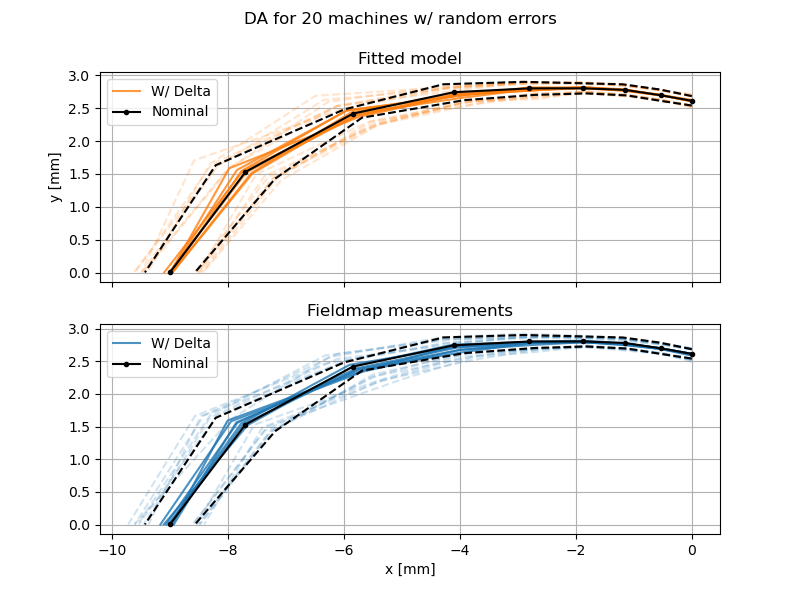
\includegraphics[width=.8\textwidth]{2023-10-27/figures/dynapt_delta.png}
        \caption{Impacto do Delta52 com magic fingers na abertura dinâmica.}
        \label{fig:dynapt}
    \end{figure}
\end{frame}

\begin{frame}{DELTA52 - Medidas de integrais (setembro)}
\begin{itemize}
        \item Medidas de integrais de campo no eixo central do ID com magic fingers.
	\end{itemize}
\begin{figure}[H]
		\centering
        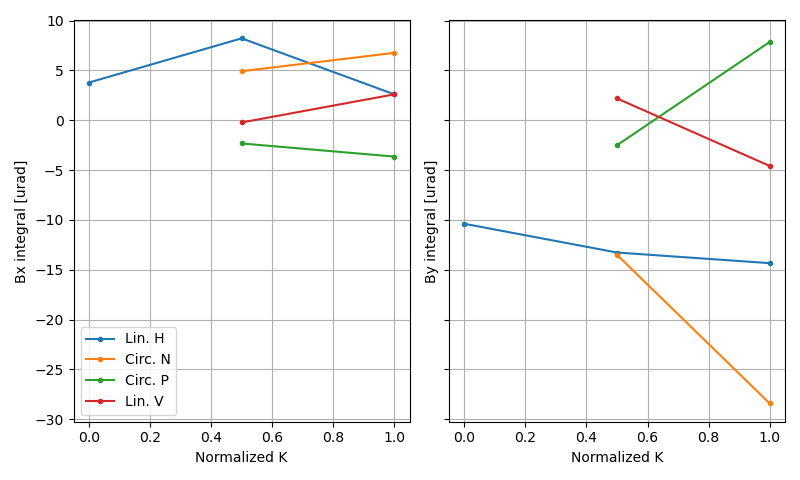
\includegraphics[width=1\textwidth]{2023-10-27/figures/field_integrals_config.png}
        \caption{Integrais de campo normalizadas pela rigidez magnética para cada configuração do Delta52.}
        \label{fig:integrals_config}
    \end{figure}
\end{frame}

\begin{frame}{DELTA52 - Medidas de integrais (outubro)}
\begin{itemize}
        \item Medidas de integrais de campo no eixo central do ID com magic fingers.
	\end{itemize}
\begin{figure}[H]
		\centering
        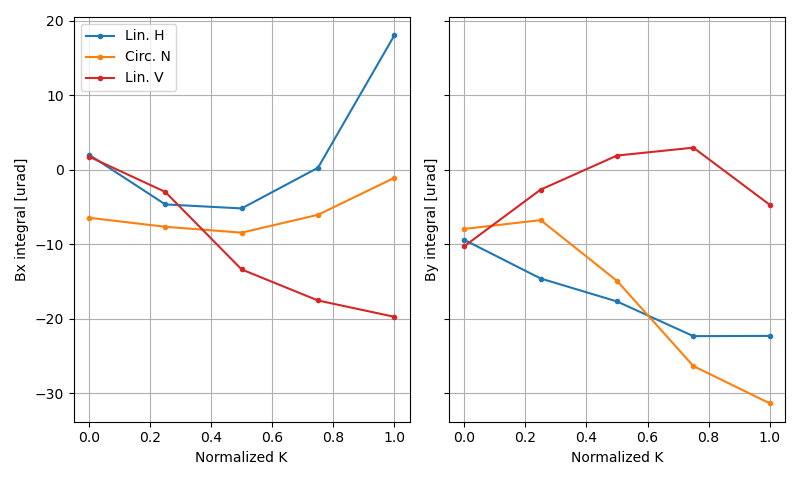
\includegraphics[width=1\textwidth]{2023-10-27/figures/field_integrals_config_new.png}
        \caption{Integrais de campo normalizadas pela rigidez magnética para cada configuração do Delta52.}
        \label{fig:integrals_config_new}
    \end{figure}
\end{frame}



\section{Atividades - Estudo de colimador para IDs}

\begin{frame}{Estudo de colimador para IDs}
\begin{itemize}
        \item Tracking do processo de perda por espalhamento Touschek (abertura física nominal).
	\end{itemize}
\begin{figure}[H]
		\centering
        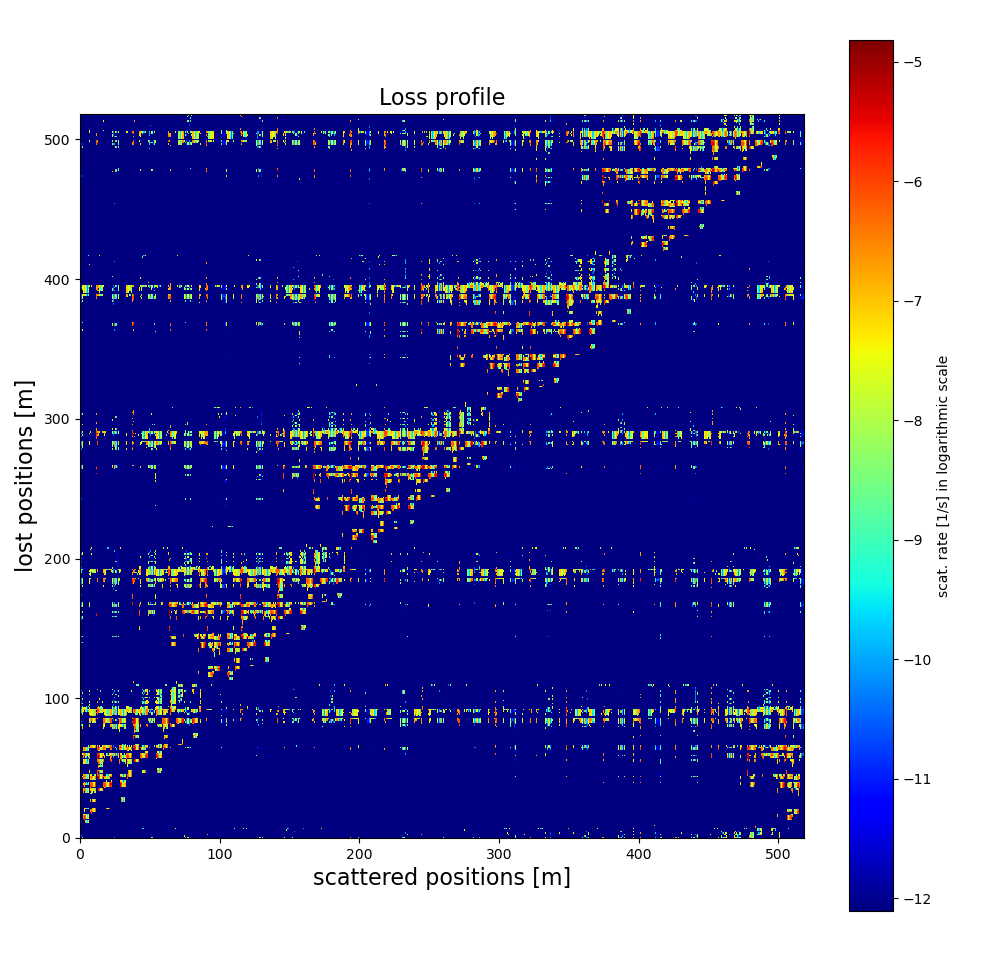
\includegraphics[width=.75\textwidth]{2023-10-27/figures/scat_vc_lost.png}
        % \caption{Comparação entre integrais de campo medidas e fornecidas pelo modelo calibrado.}
        \label{fig:scat_loss}
    \end{figure}
\end{frame}

\begin{frame}{Estudo de colimador para IDs}
    \begin{figure}[H]
    		\centering
            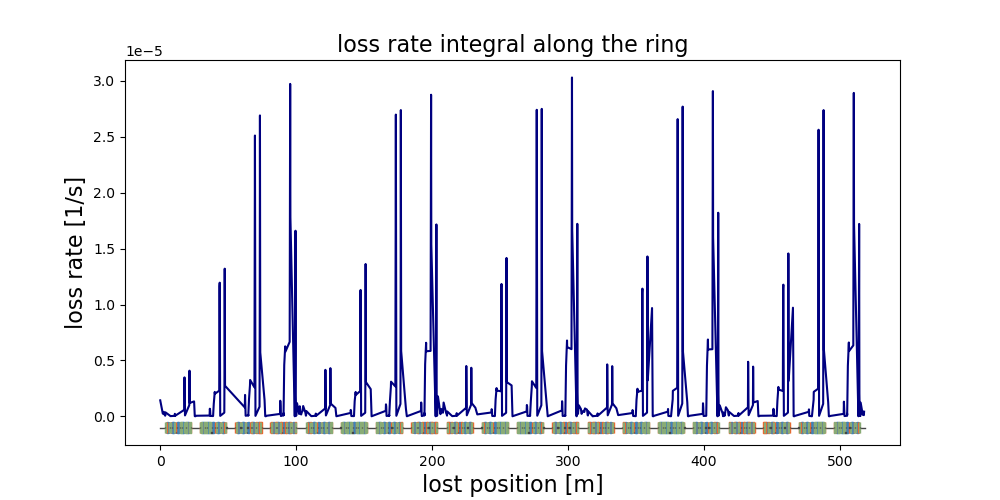
\includegraphics[width=.9\textwidth]{2023-10-27/figures/lossrate_vs_lostpos.png}
            % \caption{Comparação entre integrais de campo medidas e fornecidas pelo modelo calibrado.}
            \label{fig:scat_loss}
    \end{figure}
\end{frame}



\section{Estudos de máquina - 09/10 Scrapers}

\begin{frame}{09/10 Scrapers}
    \begin{itemize}
		\item Uso do scraper para testar a ideia de colimadores de proteção para os IDs. 
        \item Levantamos a relação entre eficiência de injeção e redução da aceitância física definida pelas fendas do scraper
	\end{itemize}
    \begin{figure}[H]
		\centering
        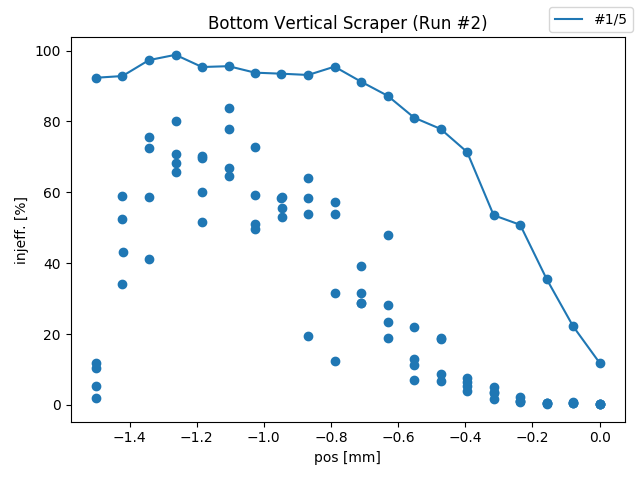
\includegraphics[width=.7\textwidth]{2023-10-27/figures/injeff-vs-vscrap.png}
        \label{fig:vgap}
    \end{figure}
\end{frame}



\section{Estudos de máquina - 09/10 Calibração VGap}

\begin{frame}{09/10 Calibração VGap}
    \begin{itemize}
		\item Continuação da medida frequência síncrotron vs. tensão de gap. Campos transversais dos IDs no mínimo e máximo (APUs, EPU e Wiggler)
        \item IDs aumentam energia perdida por volta em 28keV (+6\%)
	\end{itemize}
    \begin{figure}[H]
		\centering
        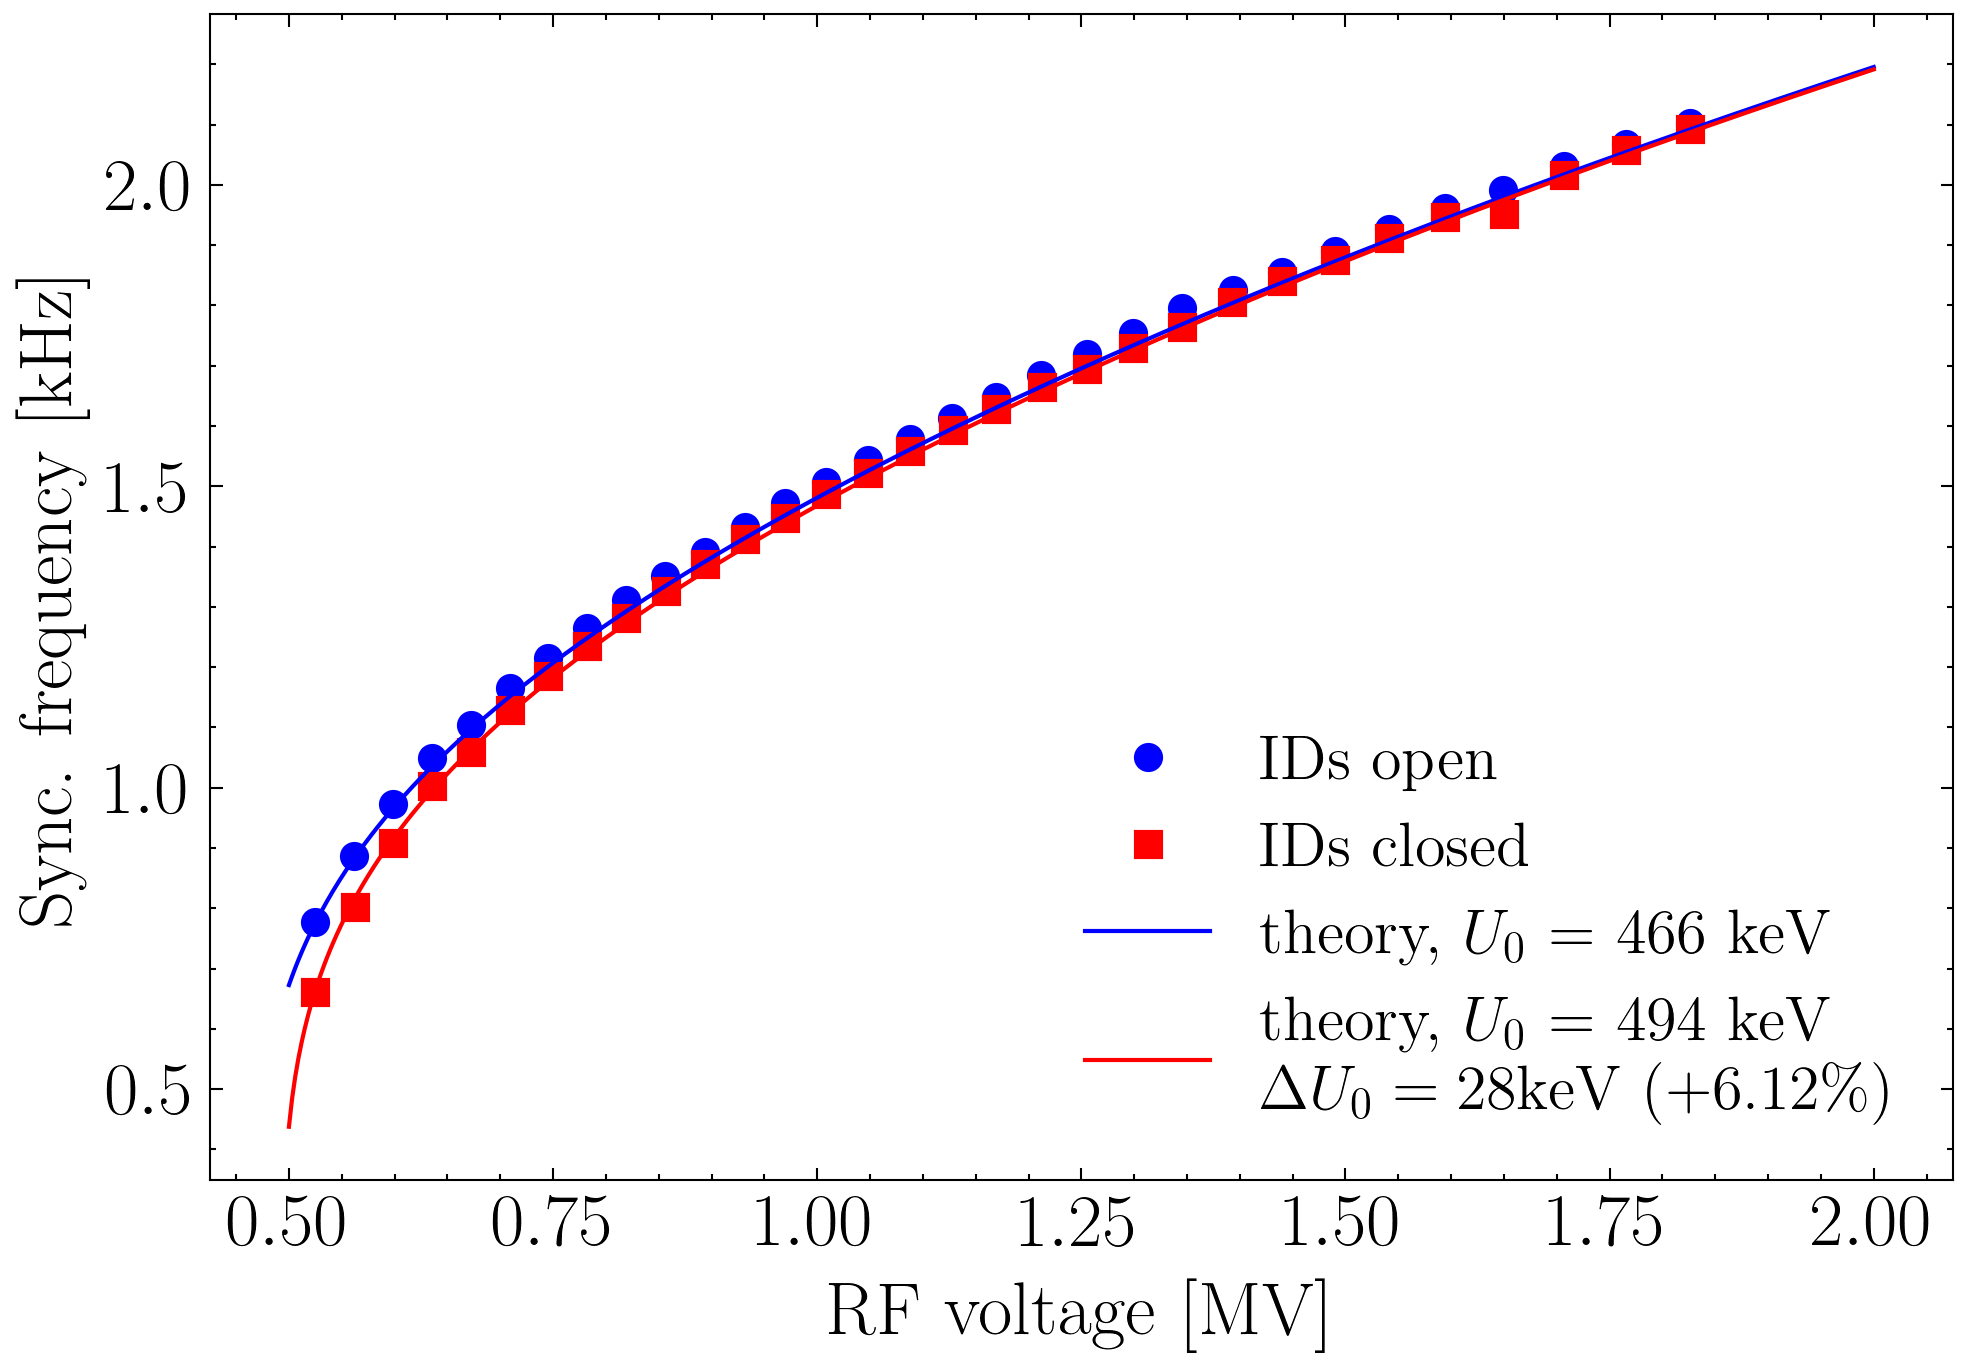
\includegraphics[width=.7\textwidth]{2023-10-27/figures/sync_freq_vs_gap_voltage_ids_variation.png}
        % \caption{}
        \label{fig:vgap}
    \end{figure}
\end{frame}



\section{Estudos de máquina - 16/10 Matriz Resposta AC}

\begin{frame}{16/10 Matriz Resposta AC}
    \scriptsize{
    \begin{itemize}
        \item Script compatibilizado com mudanças recentes nas classes de aquisição de BPMs e criação de métodos automáticos de checagem da validade dos dados medidos;
        \item Mais corretoras atuando por aquisição, medidas mais rápidas (recorde de $\sim30$ segundos)
        \item Novo procedimento de medida para coluna da RF: modulação de fase;
        \item Teste de repetibilidade da medida sob diferentes valores dos parâmetros do script:
	\end{itemize}}
     \begin{figure}[H]
		\centering
        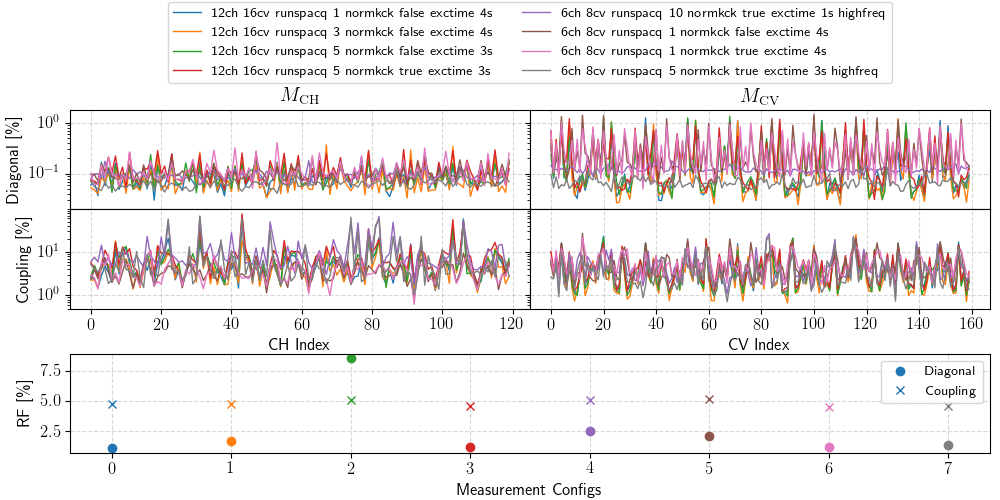
\includegraphics[width=.9\textwidth]{2023-10-27/figures/meas_repetability.png}
        \caption*{{\tiny Repetibilidade de cinco medidas para várias configurações diferentes de aquisição. A repetibilidade foi definida como desvio padrão médio de cada coluna divido pelo rms de cada coluna da matriz média.}}
        \label{fig:figure1}
    \end{figure}
\end{frame}

\begin{frame}{16/10 Matriz Resposta AC}
    \begin{itemize}
        \item Estudos sobre os ajustes dos sinais dos coeficientes dos termos fora da diagonal;
	\end{itemize}
    \begin{figure}[H]
		\centering
        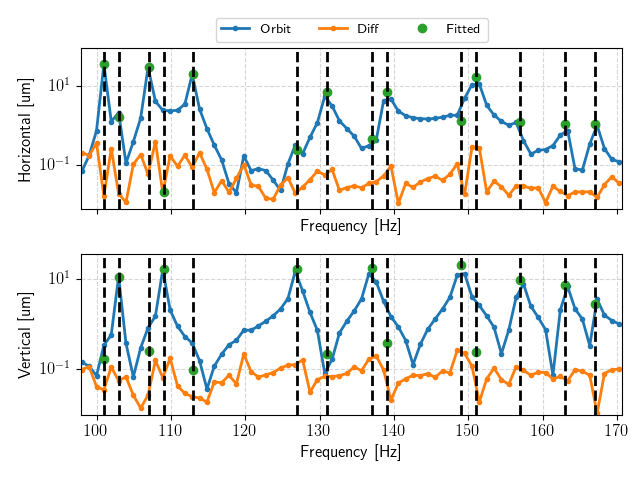
\includegraphics[width=.48\textwidth]{2023-10-27/figures/fitted_freqs.png}
        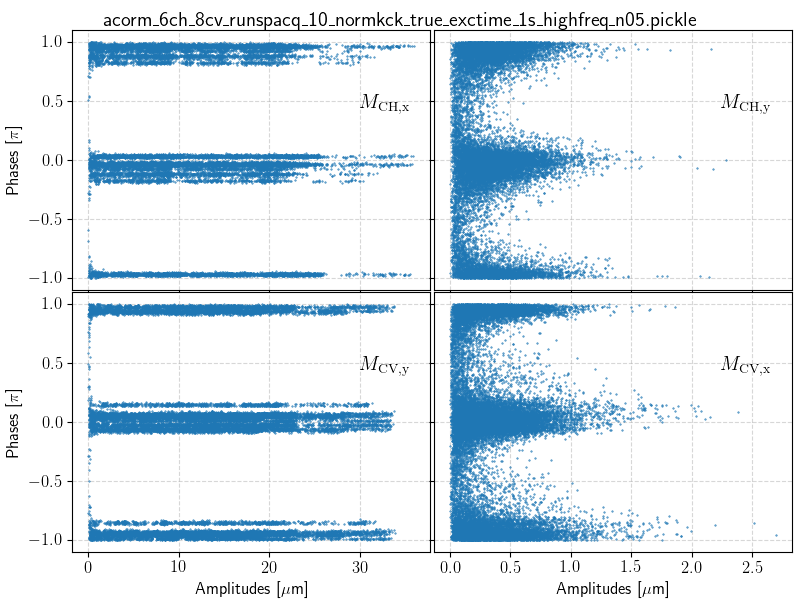
\includegraphics[width=.48\textwidth]{2023-10-27/figures/phases_vs_amplitudes.png}
        \caption*{{\footnotesize Esquerda: DFT de um BPM, mostrando as amplitudes fitadas. Direita: Phases fitadas versus amplitudes fitadas. Idealmente todas as fases deveriam ser 0 ou 1 e -1, mas para termos com pequenas amplitudes nota-se uma indeterminação da fase. Estamos estudando meios de ter mais certeza sobre esses termos}}
        \label{fig:figure1}
    \end{figure}
\end{frame}

\begin{frame}{16/10 Matriz Resposta AC}
    \begin{itemize}
        \item correção de fatores de escala (figura)
	\end{itemize}
    \begin{figure}[H]
		\centering
        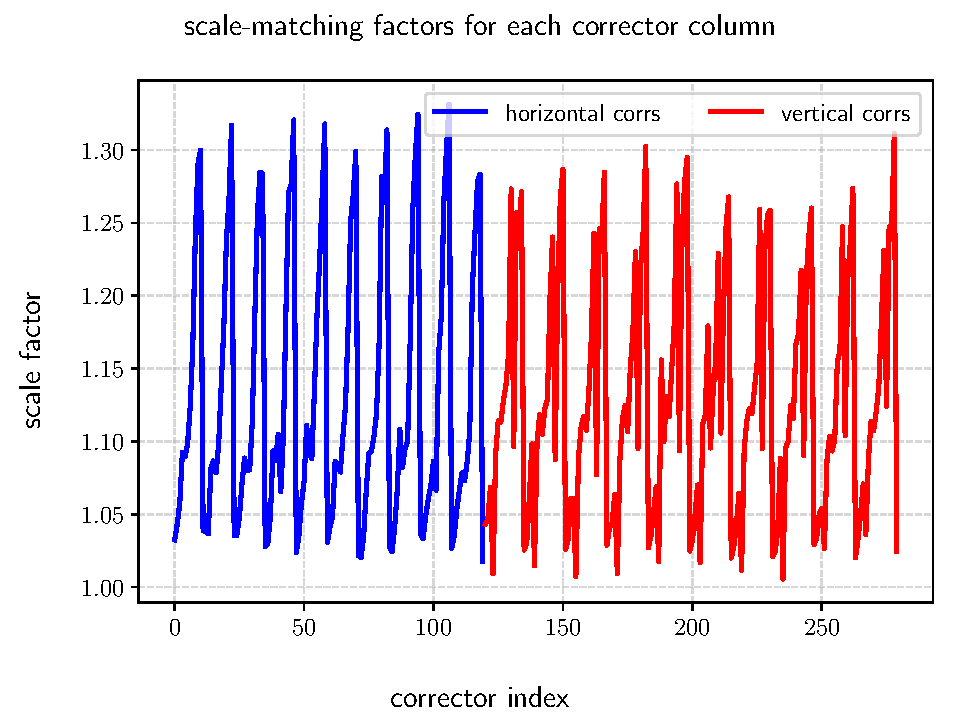
\includegraphics[width=.7\textwidth]{2023-10-27/figures/scale_factors.pdf}
        \caption*{{\footnotesize Fatores de escala (razão entre std de cols ORM DC e std de cols ORM AC)}}
        \label{fig:figure1}
    \end{figure}
\end{frame}



\section{Estudos de máquina - 17/10 Ajuste da função dispersão}

\begin{frame}{17/10 Ajuste da função dispersão}
    \begin{itemize}
		\item Correção de $\eta_y$ por desvio de órbita (vertical) nos sextupolos é equivalente a corrigir usando bobinas de quadrupolo skews nestes sextupolos.
    \begin{figure}[H]
		\centering
        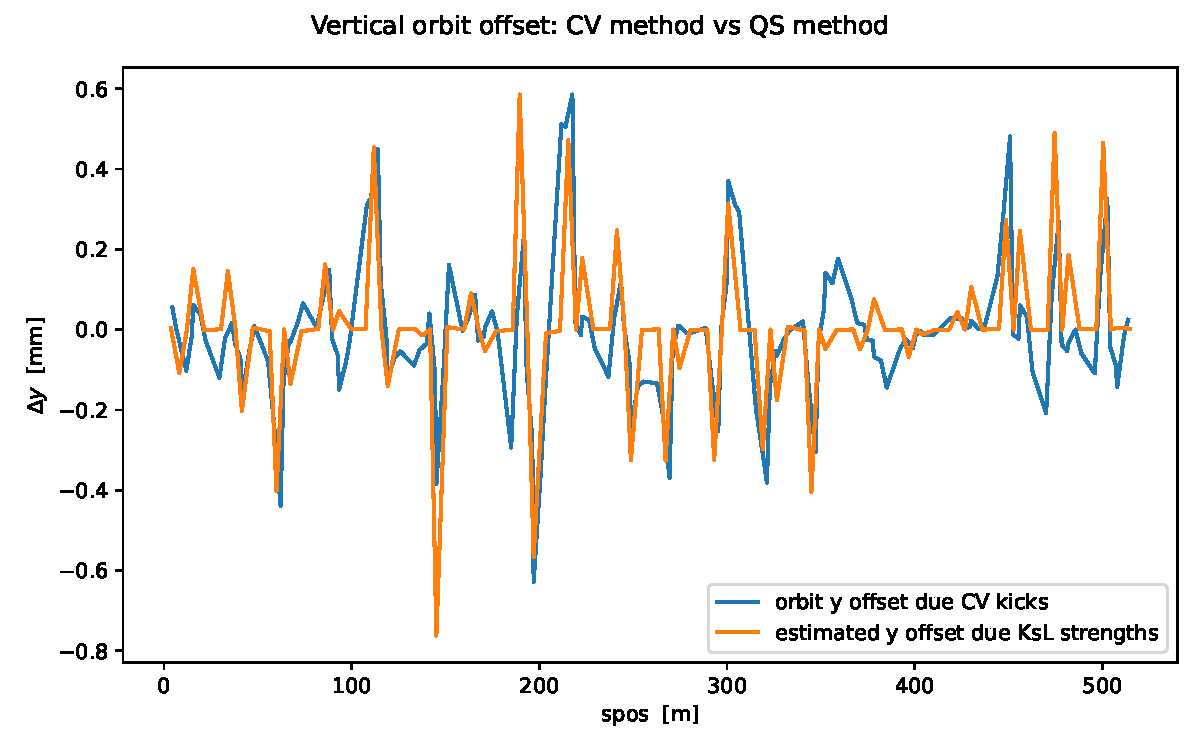
\includegraphics[width=.7\textwidth]{2023-10-27/figures/Orbit_Y_Offset_QS_versus_CV 1}
        % \caption{Dispersão vertical antes e após correção.}
        \label{fig:figure1}
    \end{figure}
	\end{itemize}
\end{frame}

\begin{frame}{17/10 Ajuste da função dispersão}
    \begin{itemize}
        \item Fizemos correção de $\eta_y$ com quad. skew dos sextupolos cromáticos (60 sgvs da matriz total).
        \item Redução de um fator $\sim$~8 no pico-a-pico de $\eta_y$ residual
    \begin{figure}[H]
		\centering
        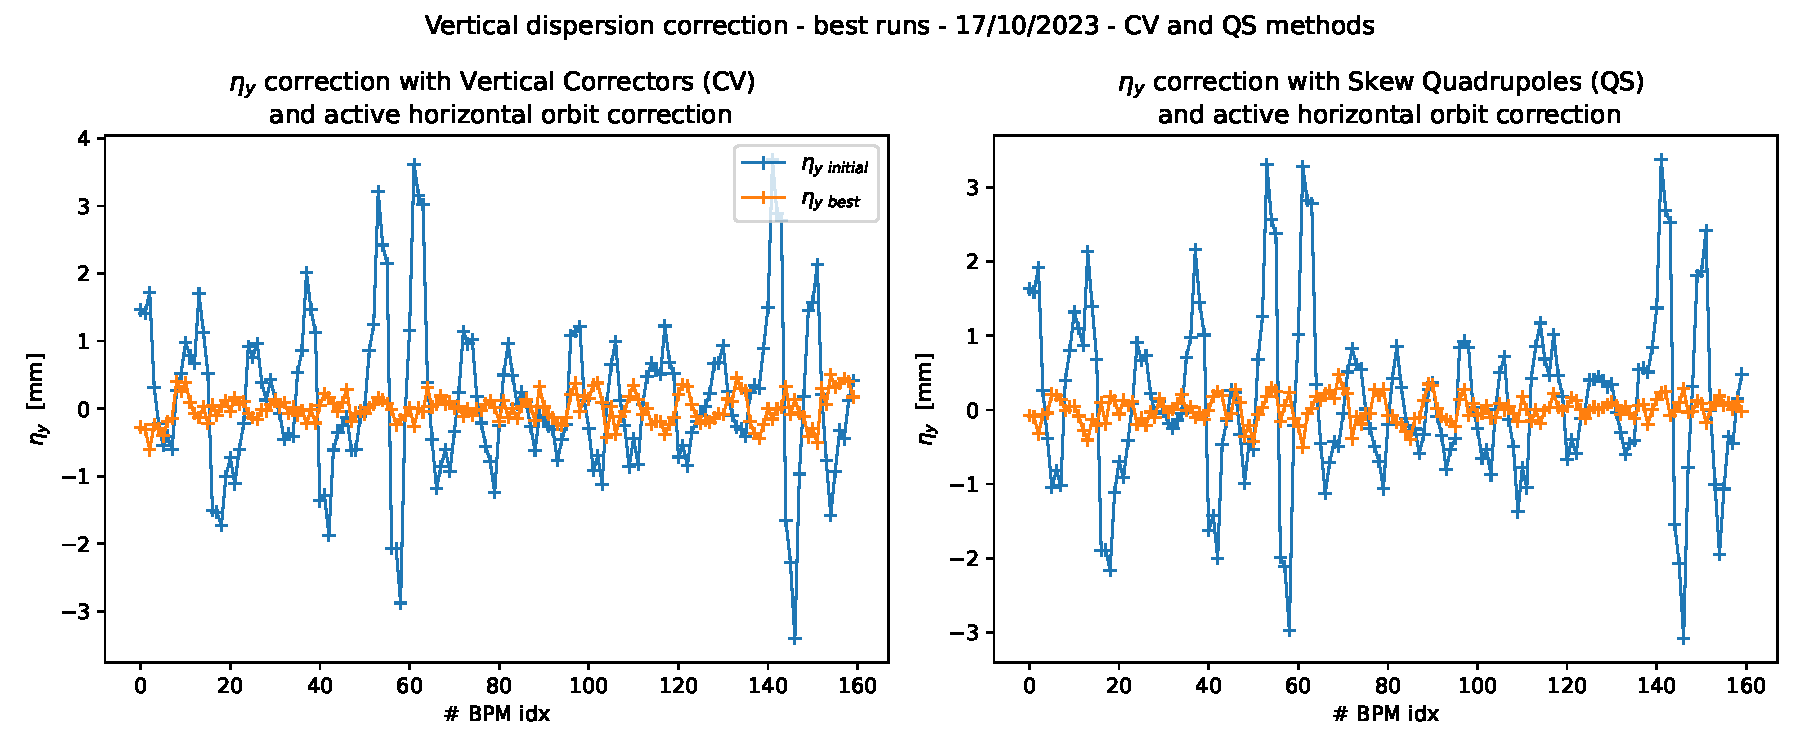
\includegraphics[width=0.92\textwidth]{2023-10-27/figures/Vertical_dispersion_correction_with_CV_and_QS_methods_day17 1}
        % \caption{Dispersão vertical antes e após correção.}
        \label{fig:figure1}
    \end{figure}
	\end{itemize}
\end{frame}

\begin{frame}{17/10 Ajuste da função dispersão}
    \begin{itemize}
        \item Após a correção o acoplamento aumentou para algo em torno de 2\%.
        \item Corrigimos acoplamento na respmat (medida AC) usando como botões LOCO os skews acromáticos. Acoplamento pelo modelo calibrado: $\sim$ 0.2\%.
        \item Controlamos o acoplamento usando skews não dispersivos (padrão) observando o tamanho vertical na CAX. O ângulo aumentou de 0° para 4°.
    \begin{figure}[H]
		\centering
        \includegraphics[width=.9\textwidth]{2023-10-27/figures/beam_view 1}
        \label{fig:figure1}
    \end{figure}
	\end{itemize}
\end{frame}



\section{Estudos de máquina - 23/10 Estudos com a Carnaúba}

\begin{frame}{23/10 Estudos com a Carnaúba}
    \begin{itemize}
        \item Medidas simultâneas com feixe de elétrons na sala de controle e feixe de fótons na linha de luz
        \item Medidas na linha feitas com taxas de aquisição diferentes (2kHz e 2.5kHz), apenas algumas frequências no espectro mudaram, nenhuma das frequências relevantes foi afetada
        \item Medidas com FOFB on e off. 60Hz é atenuado por fator 10 pelo FOFB, no anel e na linha. FOFB também atenua bem 15Hz, perceptível na linha. FOFB off + rampa ligada tem bastante efeito na linha, múltiplos de 2Hz.
        \item Outras frequências com amplitude grande, 54Hz, 89Hz, (...) não são afetadas pelo FOFB. Indicativo de ser devido ao espelho
	\end{itemize}
\end{frame}





\section{References}



\end{document}
